\section{Background}

\subsection{Artificial Neural Networks}
Neural networks are a type of model that is based on the way that brains function. Artificial neural networks are made up of components called neurons which are stacked into layers and connected to form a network. Neural network operation consists of providing input data to the input layer of the network, passing that data along to network to the output layer and then interpreting the output in a specific way. In the case of predator vs prey, output neurons will correspond to different actions that the predator and prey can make.

\subsubsection{Neurons}
As mentioned above, the key components of a neural network is the neuron. The sole job of the neuron is to compute the weighted sum of all of the inputs to the neuron and then proceed to pass the value through an activation function. For the purposes of this paper the logistic function as seen in figure \ref{fig:sigmoid} represented by the equation \ref{eqn:sigmoid}.

\begin{equation}
	    y = \frac{1}{1+e^(-x)}
	    \label{eqn:sigmoid}
\end{equation}


\begin{figure}
  \centering
  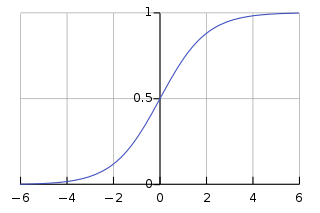
\includegraphics[width=0.5\textwidth]{sigmoid.png}
  \caption{Graph of logistic function}
  \label{fig:sigmoid}
\end{figure}





\subsection{Particle Swarm Optimization Overview}
Particle swarm optimization(PSO) was developed by Kennedy and Eberhart (1995). PSO takes inspiration from the flocking behavior of swarms of birds. When observing birds there tends to be one leader and the rest of the flock tend to follow that leader. Particles which are analogous to birds are spread throughout a solution space where the particle with the best solution to the problem becomes the leader (global best). Throughout multiple generational time steps the rest of the particles converge towards the global best. If a new best solution is found, the particle that found the new best solution becomes the global best and the process continues until convergence or a max generation cap is reached.

\subsection{Vanilla PSO}
\subsubsection{Particles and Swarms}
As mentioned above, a particle is the base unit of the PSO. Particles consist of a location in the solution space, a velocity and a fitness which is used to determine the best particle. A group of particles make up a swarm. The global best is determined within a swarm, thus if multiple swarms are used each swarm could potentially have a different global best.
	
\subsubsection{ Particle Update}
	An update of a particles location consists of several terms. As convergence is expected, naturally a component of the update is towards the global best. This is called the social term. Another component is the draw towards the particles best seen location (local best). This is called the cognitive term. Each of these terms has a corresponding co-efficient which can be adjusted based on what is required from the PSO. Coefficients tend to be picked based on graph \ref{fig:pso-convergence} that was proven to be convergent by \cite{englebrecht-pso}. A velocity update can be made by combining the social and cognitive terms using the following equation:
	
\[ v(t+1) = \omega * v(t) + c_1*\psi_1 * (p(t) - x(t)) + c_2*\psi_2 * (g(t) - x(t)) \] Where,\\
\indent $v$ is the velocity of the particle\\
\indent $c_1$ and $c_2$ are the personal and social coefficients respectively\\
\indent $\psi$ is a random multiplier between 0 and 1\\
\indent $x(t)$ is the location of the particle at time t\\
\indent $p(t)$ is the personal best location of the particle at time t\\
\indent $g(t)$ is the global best location of the swarm at time t\\
	
The updated velocity is then used to update the position of the particle. The outline of the steps required to implement the PSO can be found in figure \ref{fig:pso-pseudocode}.


\begin{figure}
  \centering
  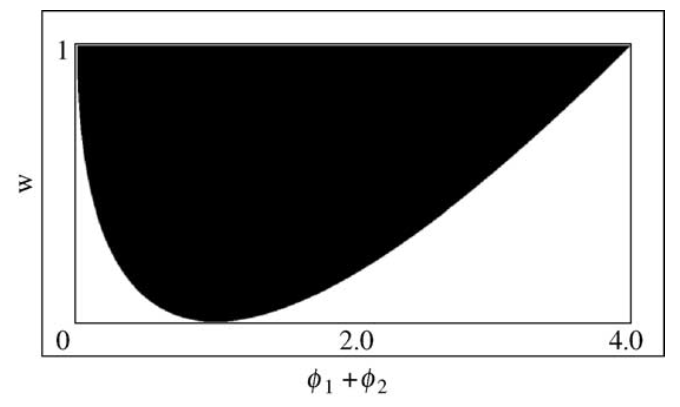
\includegraphics[width=0.5\textwidth]{pso-conv.png}
  \caption{Parameter convergence graph for PSO}
  \label{fig:pso-convergence}
\end{figure}

 
\begin{figure}
  \centering
  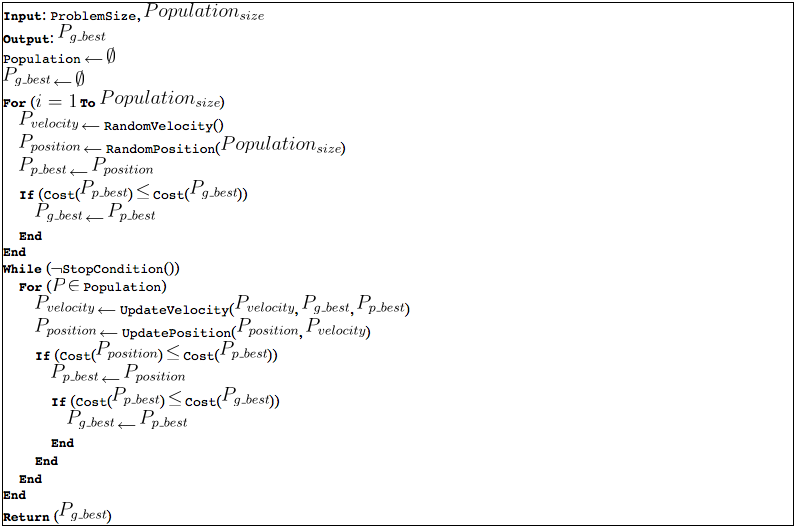
\includegraphics[width=0.8\textwidth]{pso-pseudocode.png}
  \caption{PSO Pseudocode}
  \label{fig:pso-pseudocode}
\end{figure}


\subsection{Charged PSO}
	Charged PSO differs slightly form the vanilla PSO. Charged PSOs have swarms as well, however in these swarms a particle has a change to be charged. If two charged particles are too close to each other, a repulsive force will be added to the velocity update function. This prevents total convergence allowing for the continuous searching of the search space. Charged PSOs are used in dynamic environments where a complete convergence could allow for a non-optimal solution. Thus to ensure that the solution develops along with the changing error landscape total convergence is actively prevented by the use of these charged particles. The updated velocity function for charged particles is as follows:
	
	
\[ v(t+1) = \omega * v(t) + c_1*\psi_1 * (p(t) - x(t)) + c_2*\psi_2 * (g(t) - x(t)) + a_i(t)\]

with  \[ a_i(t) = \sum_{j=1, j\neq i}^{n_s} a_{ij}(t) \] Where,

\[a_{ij} = 
\begin{cases}  
\frac{Q_{i}Q_{j}}{d_{ij}^3} * (x_{i}(t)-x_{j}(t)) & \text{if} R_{c} \leq d_{il} \leq R_{p}\\ 
\frac{ Q_{i}Q_{j} }{d_{ij}^3}*(x_{i}(t)-x_{j}(t)) & \text{if} R_{c} < d_{il} < R_{p}\\ 
0 & \text{otherwise}
\end{cases}\] Where,\\
\indent $d_{ij} = ||(x_{i}(t)-x_{j}(t))||$\\
\indent $Q$ is the charge of the particle \\
\indent $R_{c}$ is the core radius \\
\indent $R_{p}$ is the particle perception limit
